\subsection{ERD Diagram}

\begin{figure}[H]
    \centering
    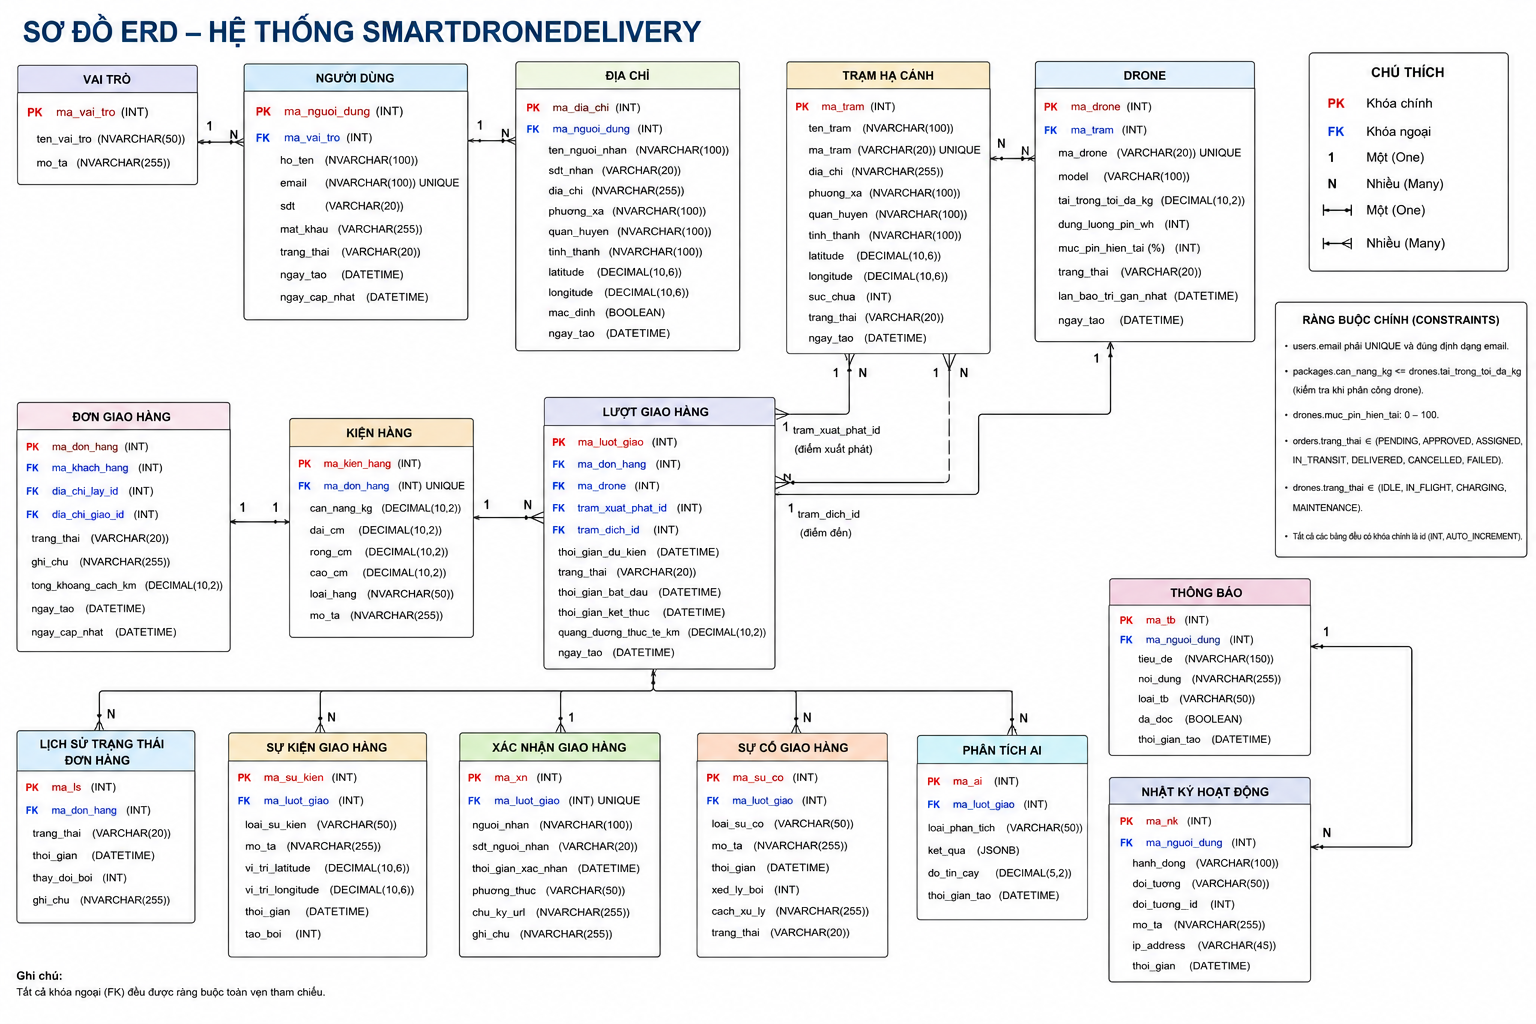
\includegraphics[width=\linewidth]{images/Sơ đồ ERD.png}
    \caption{Sơ đồ ERD của hệ thống}
    \label{fig:erd}
\end{figure}

Sơ đồ ERD mô tả các quan hệ chính của hệ thống. Một người dùng có thể sở hữu nhiều địa chỉ và nhiều đơn hàng; mỗi đơn hàng có thể chứa một hoặc nhiều kiện hàng, được theo dõi qua lịch sử trạng thái. Đơn hàng được gắn với chuyến giao, lịch giao, drone và trạm hạ cánh trong quá trình điều phối.

Các bảng \texttt{delivery\_events}, \texttt{order\_status\_history} và \texttt{activity\_logs} có vai trò lưu vết thay đổi theo thời gian. Nhóm bảng này không thay thế dữ liệu hiện tại trong các bảng nghiệp vụ mà bổ sung bằng chứng về thời điểm, tác nhân và nội dung thay đổi.